\documentclass[tcc]{subfiles}

\begin{document}

\chapter{Methods}
\label{sec:methods}
\epigraph{It's not denial. \\ I'm just very selective about the reality I accept.}{-Calvin}

This section deals with the models used for the engine compressor, turbine and nozzle, 
as well as the methods used for calculating the engine steady operation (engine matching), 
surge, dynamical behavior and performance parameters. 
Throughout this section, the ideal gas assumption is widely used, 
as is the assumption that the performance of a component can be separated in an ideal performance and a loss model. 
In the end, the engine from which the parameters for the model were extracted is described.

The component models are normally referred to as component maps or characteristic lines. 
A component map or characteristic is, in a general sense, the functional relationship between a component's
mass flow rate, rotation speed, pressure ratio and efficiency. 
These five unknowns are linked by two constraints, namely Euler's equation and a loss model. 
This leaves two free variables, i.e.\ a two dimensional set of solutions.
Usually compressor maps are plotted using the mass flow rate as the abscissa and  the pressure ratio as the ordinate, with contours for constant rotation speed and efficiency. 
For turbines, the rotational speed and efficiency is not uniquely defined for a combination of mass flow rate and pressure ratio. This led to the use of the artificial parameter of rotational speed times mass flow rate for the abscissa.

The name characteristic is most often used in reference to the iso-speed lines of a turbine or compressor when plotted in the plane of flow parameter vs.\ pressure ratio.
For incompressible flow this leads to the collapse of the constant rotational speed lines, thus being very convenient.

\section{Compressor model}

\subfile{text/body/compressor_map}

To write Euler's equation \cref{eqn:euler} in terms of the nondimensional parameters introduced in \cref{sec:nondimensional}, it suffices to rewrite $\phi_3$ and $\psi$ as a function of them. Thus
\begin{multline}
    \label{eqn:phi2_dimensionless}
    \phi_3 = \frac{W_{2r}}{U_3} 
           = \frac{\frac{\dot{m}}{\rho_3 A2}}{\acs{M0rotor} a_{02}}
           = \frac{\MFPalt{2}}{\acs{M0rotor}} \frac{a_{03}}{a_{02}} \stagdensratio{3} \\ 
           = \frac{\acs{MFP}_3}{\acs{M0rotor}} \sqrt{\frac{T_{03}}{T_{01}}} \stagdensratio{3}
\end{multline}
The value of $M_3$ can be obtained from $\acs{MFP}_3$ using \cref{eqn:mfp2mach}, while the latter is given by
\begin{equation}
    \label{eqn:mfp2mfp2}
    \acs{MFP}_3 \triangleq \MFP{2} = \acs{MFP} \frac{A_2}{A_3} \frac{P_{02}}{P_{03}} \sqrt{\frac{T_{03}}{T_{02}}}
\end{equation}
Notice that \cref{eqn:mfp2mfp2} makes no assumption of the process 1--2 being isentropic. Furthermore $\acs{MFP}_3$ can be used along with $\acs{MFP}_2$ to check for choking.

Finally, the load coefficient is given by
\begin{equation}
    \acs{load_coef}\triangleq \frac{\Delta h}{U_3^2}
                      = \frac{c_p(T_{02}-T_{02})}{U_3^2}
                      = \frac{\frac{c_p(T_{03}-T_{01})}{\gamma R T_{02}}}
                                    {\acs{M0rotor}^2}
                      = \frac{\frac{T_{03}}{T_{02}}-1}
                                  {\acs{M0rotor}^2}
                        \left(\frac{1}{\gamma-1}\right)
\end{equation}

At this point the loss models discussed in \cref{sec:compressor_losses} are introduced, 
and the values of $\acs{load_coef}_{\text{actual}}$ and $\acs{load_coef}_{\text{isen}}$ are obtained.
The temperature and pressure ratios can then be readily calculated from
\begin{align}
    \label{eqn:psi2Tratio}
    \frac{T_{03}}{T_{02}} &= (\gamma - 1)\psi_{\text{actual}} \acs{M0rotor}^2 + 1 \\
    \label{eqn:psi2Pratio}
    \frac{P_{03}}{P_{02}} &= \left[(\gamma - 1)\psi_{\text{isen}} \acs{M0rotor}^2 + 1\right]^\frac{\gamma}{\gamma-1}
\end{align}

In this work, only the losses due to incidence and skin friction were considered, because they are the ones most important for compressor stability. The model chosen for skin friction was the one selected by the comparative study of \textcite{Oh1997} and the incidence losses where modeled as the complete conversion of all kinetic energy normal to be blade camber line to heat \cite{Galvas1973}, i.e.\
\begin{align}
    \Delta \psi &= \left[\left(\frac{r_3}{r_2}\right)^2 + \phi_2^2\right]
    \sin(\beta_2 - \beta_{2\text{opt}}) \quad\text{for the inducer} \\
    \Delta \psi &= (\psi_{\text{euler}}^2 + \phi_2^2) \sin(\alpha_3-\alpha_{3\text{opt}}) \quad\text{for the vanned diffuser}
\end{align}
where $\beta_2$ and $\alpha_3$ are the actual blade (metal) angles and $\beta_{2\text{opt}}$ and $\alpha_{3\text{opt}}$ are the flow angles for each flow condition.

This is a more physical model than the one suggested by Oh et al., and captures better the loss variation with incidence, since Oh et al's model does not include flow angles. 

The compressor model is summarized in \cref{map:compressor}.

\section{Turbine model}
\subfile{text/body/turbine_map}

The turbine model is summarized in \cref{map:turbine}. 
Its development is mostly analogous to that of the compressor, with the exception of the loss and deviation models. 
Since the turbine does not exhibit flow instability phenomena such as compressor surge, 
which depends heavily on the incidence losses, 
the turbine was assumed isentropic. 
Nevertheless, a loss model based on pressure loss coefficients $Y_p$, $Y_s$, $Y_k$, etc.\ 
could easily be included in this model by modifying \cref{eqn:turb_res_pr} in the following way
\begin{equation}
    \frac{P_{05}}{P_{04}} -\frac{[1 + (\gamma-1)\psi_{\text{euler}} M_b^2]^{\frac{\gamma}{\gamma-1}}}{1+Y\left\{1-\left[1+\tfrac{\gamma-1}{2}M_5^2\right]^{-\frac{\gamma-1}{\gamma}}\right\}} = 0 
\end{equation}
where
\begin{equation}
    Y = Y_p + Y_s + Y_k
\end{equation}

This correction is derived as follows. The pressure loss coefficient is given by
\begin{equation}
    Y = \frac{P_{0i} - P_{0e}}{P_{0e} - P_e}
\end{equation}
Now we divide the numerator and the denominator by $P_{0e}$ and isolate the pressure ratio term 
\begin{equation}
    \frac{P_{0i}}{P_{0e}} = \frac{1}{1+Y\left\{1-\left[1+\tfrac{\gamma-1}{2}M_e^2\right]^{-\frac{\gamma-1}{\gamma}}\right\}}
\end{equation}
This pressure ratio loss term must be multiplied to the ideal (isentropic) pressure ratio given by the second term of \cref{eqn:turb_res_pr}. If more than one blade row is considered (e.g.\ one for the stator and another one for the rotor) the pressure ratio losses ($Y$) for each must be joined by multiplication.

\subfile{text/body/nozzle}


\section{Engine static model}
\label{sec:model:static}

The engine static model, also known as the matching model, 
describes the conditions in which the engine can operate indefinitely 
without changes in throttle input or outside conditions (pressure and temperature).

The engine model used is of the lumped volume type. This means that each component 
 (compressor, burner,turbine and nozzle)
 is modeled as a single point in space and conservation laws are applied to them.
 This type of model is also known as zero dimensional (0-D) or as parametric cycle analysis
 \index{parametric cycle analysis},
 and is widely used in both industry and academy as a tool for preliminary design and 
 performance analysis. 

A schematic of the engine components considered for the simulation of the present gas turbine engine is shown in \cref{fig:engine_schematic}.

The model was derived considering following constraints:

\begin{enumerate}
    \item conservation of energy through the spool, \cref{eqn:engine:energy};
    \item conservation of mass in the burner, \cref{eqn:engine:mass};
    \item conservation of energy in the combustion process, \cref{eqn:engine:burn};
    \item the nozzle equation, \cref{eqn:nozzle};
    \item and the compressor and turbine models, \cref{map:compressor,map:turbine}.
\end{enumerate}

This model is shown in \cref{map:engine}. It has 12 variables and 11 equations, so it has a one dimensional solution set i.e. the work line.
\subfile{text/body/engine_map}

\section{Engine dynamical model}
The dynamical engine model adopted was the one described in \cref{sec:review:dynamics}. It is similar to the one described in \cref{sec:model:static} with the following changes:

\begin{enumerate}
    \item The conservation of energy in the spool, \cref{eqn:engine:energy}, is replaced by \cref{eqn:dynamic:energy} to allow spool acceleration;
    \item The conservation of mass in the burner, \cref{eqn:engine:mass}, is replaced by \cref{eqn:dynamic:mass}  to allow transient changes in density within the burner;
    \item The implicit assumption that the pressure in the burner is constant from inlet to exit ($P_{03}=P_{04}$) is dropped and replaced by the conservation of momentum in the combustion chamber, \cref{eqn:dynamic:momentum};
    \item and the ideal gas equation is added to link the pressure, density and temperature in the combustion chamber.
\end{enumerate}

This results in the nonlinear system shown in \cref{model:dynamic}. It has 14 variables and 13 equations, thus it is a single input system, like the static model. For a control problem, the input variable would be the fuel mass flow.

\subfile{text/body/dynamical_map}

\section{Surge model}

Due to the nonavailability of an off the shelf partial \ac{DAE} solver, the model described in \cref{sec:review:surge} was not implemented. Instead, the surge line was estimated to be at a \acs{MFP} equivalent to 80\% of the required \acs{MFP} to achieve minimum angular speed for a given pressure ratio, i.e. 20\% before the peak of the compressor characteristic. 
To implement \cref{sec:review:surge}'s model in a partial \ac{DAE} or with discretized partial derivatives, the static model (\cref{sec:model:static}) could be used with the nozzle equation, \cref{eqn:nozzle}, removed since for surge it is important to consider the engine at any overall pressure ratio ($\pr{05}{02}$). The addition of the stability criteria would maintain the number of equations, thus the solution set would still be a line.

\section{Numerical aspects}

As was shown in this section, the models for a gas turbine engine and its components are expressed naturally in the form of coupled (sometimes differential) non-linear systems of equations. 
These systems are inherently coupled because their behavior depends on the flow angles on both the inlet and exit, and these can not be calculated independently of one another.
As discussed in \cref{sec:review:numeric}, these problems are examples of \ac{DAE} systems, and many of them do not have explicit derivatives in their formulation.

In this section, the numerical approach used to calculate each of the models described in this chapter will be exposed. They consist of a mix of nonlinear solvers, namely Powell's hybrid method and Levenberg-Marquardt, as implemented by \textsc{minpack} and available in the Python package scipy, and of the newer \ac{DAE} solver \textsc{IDA}, available as part of \textsc{sundials} \cite{sundials} with a Python interface by Assimulo \cite{assimulo}.

\subsection{Generation of component maps}
A classic nonlinear solver was used, coupled with a breadth-first search approach for propagating previous solutions as initial guesses. 
Firstly, the initial point in the $x$ and $y$-axis is chosen randomly within the choke boundaries, 
pressure and temperature ratios are unit, mach numbers are between 0 an 1. 
If convergence is achieved a breadth-first search considering that each point in the grid is a graph node connected to the points up, down, left, right and in the diagonals is done.
Considering this search tree, the solution for each parent is used as a initial guess for its children. Provided that the grid is thin enough, this provides very good initial guesses for the nonlinear solver, ensuring fast and robust convergence. Furthermore, since each node has 8 neighbours, they can have up to 8 different initial guesses, which makes this approach even more robust.

\subsection{Choke line}
Drawing the choke line for the compressor is generally straightforward, since it is practically linear. The first step is to find the point where inlet and exit are simultaneously choked. For pressure ratios above this critical value, only the inlet is choked and the choke line is vertical. For pressure ratios bellow this value the exit is choked. The choke line was verified to be a straight in this region, so that just solving for a choked point at another pressure ratio, e.g.\ the minimum pressure ratio of interest (normally unit) is needed to fully define it.


Drawing the line for the turbine is slightly more elaborate, because although it is linear in a plot of \acs{MFP} vs.\ pressure ratio it is not in a plot of $\acs{MFP}M_b$ vs.\ expansion ratio.
For the particular turbine used in this work, the choke was found to be determined by the turbine exit, so this was the condition checked. After a initial point on the choke line was found, it was used as a initial guess for finding the next. This approach, however, is not very robust. We recommend instead using a KS aggregation function to join the two choke conditions in one equation, and then use a path following solver to find the choke line \cite{martins}.

\subsection{Generation of the working line}
We recommend firstly optimizing the engine model for maximum efficiency, subject to the model constraints. In general high efficiency points are more linear, so convergence is facilitated.
After that, use a \ac{DAE} solver to continue the line forwards and backwards.

\section{The VT-80 engine}
The engine chosen to which apply these models was Jet-Munts VT-80.
This engine was developed for hobby use in airplane models. It is a 
It is a single spool jet engine, with a single stage centrifugal compressor 
 and also single stage axial turbine, as seen in \cref{fig:engine}. It stems from the original micro turbine desin by \textcite{Schreckling1994} and improved by \textcite{Kamps1999}, among others. 
It runs on aviation kerosene premixed with oil.
The specifications provided by the manufacturer are in \cref{tbl:engine_specs}.
\textcite{bolsoni} estimates the compressor pressure ratio 
to be around 2.2 based on similar engines. Engines and components drawings with all dimensions relevant for the simulations are annexed to this work. This drawings were based on Kamps' design, measurements of the actual engine, and CAD models found online.

\begin{figure}[p]
    \centering
    \caption{JetsMunt VT-80 jet engine}
    \label{fig:engine}
    \begin{subfigure}{\textwidth}
        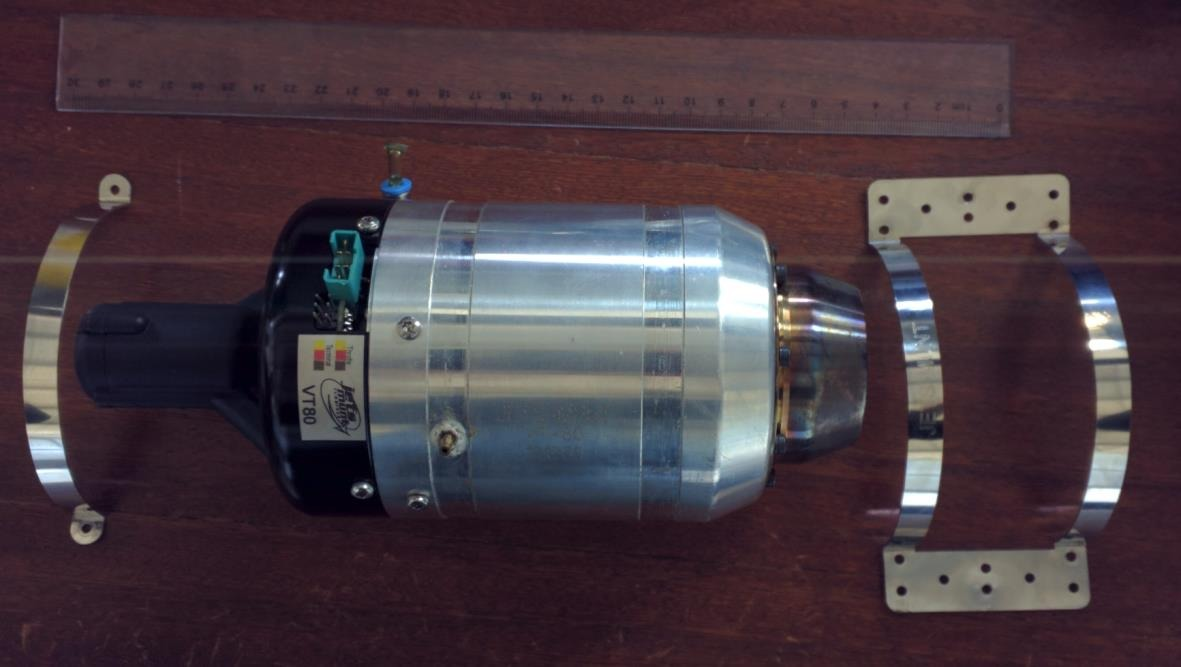
\includegraphics[width=\textwidth]{fig/JetsMuntVT-80.jpg}
        \caption{Picture with a 30cm ruler for scale}
        \label{fig:engine!visible}
    \end{subfigure}
    \begin{subfigure}{\textwidth}
        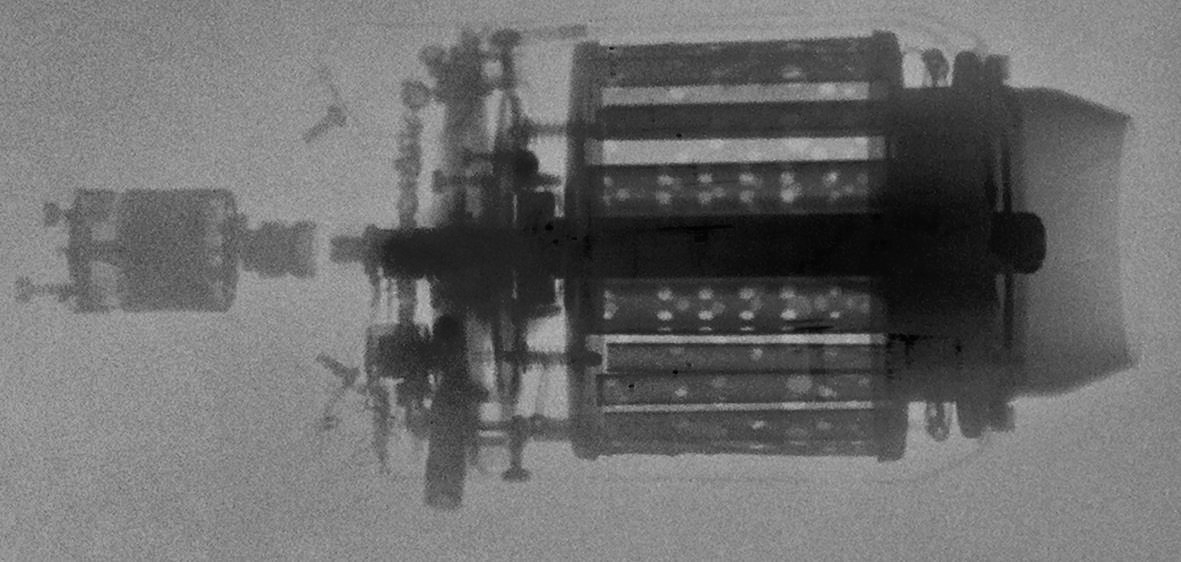
\includegraphics[width=\textwidth]{fig/JetsMuntVT-80X-ray_enhanced.jpg}
        \caption{X-ray picture}
        \label{fig:engine!x-ray}
    \end{subfigure}
    \source{\cite{bolsoni}}
\end{figure}

\begin{table}
    \centering
    \caption{VT80 Specifications}
    \label{tbl:engine_specs}
    \begin{tabular}{lr@{$\,$}l}
        \toprule
        Diameter (external)                & 90 & mm \\
        Length                             & 240 & mm \\
        Weight (bare)                      & 950 & g \\
        Weight (with accessories)          & 1075 & g \\
        Nominal thrust @ 15C and sea level & 80 & N \\
        Idle thrust                        & 4 & N \\
        Max rpm                            & 150 000 & rpm \\
        Idle rpm                           & 45 000  & rpm \\
        Heat soak rpm                      & 12 000  & rpm \\
        \acs{EGT} @ max rpm                & 600$\pm$50 & \si{\celsius} \\
        Fuel consumption @ max rpm         & 0.29 & L/min \\
        Fuel/oil                   &\multicolumn{2}{l}{Kerosene + 4\% oil} \\
        \bottomrule
    \end{tabular}
    \source{\cite{engine-manual}}
\end{table}

\end{document}
